\chapter{El algoritmo}

% TODO: escribir la idea general

\noindent
En este capítulo desarrollamos el algoritmo para resolver prácticamente cualquier tipo de problemas
de programación lineal entera; se divide en tres subsecciones que construyen el algoritmo de forma
incremental. En primer lugar, consideramos el caso cuando las únicas dos restricciones son de no
negatividad ($\vec{x} \geq \vec{0}$) y una presupuestaria ($\vec{c}^T\vec{x} \leq u$ para algún
escalar $u$). A partir de ello, generamos una sucesión de ecuaciones lineales enteras cuya solución
provee candidatos para el óptimo del problema.

En segundo lugar, agregamos $m$ restricciones de desigualdad además de la presupuestaria. Este es el
parteaguas donde el algoritmo toma relevancia, pero donde también aumenta en complejidad y supone
ciertas dificultades con los tiempos de terminación. Discutiremos ampliamente posibles direcciones
que puedan mejorar de manera significativa la rapidez de nuestro algoritmo.

En tercer lugar, eliminamos la restricción presupuestaria y, por lo tanto, nuestro algoritmo será
capaz de resolver problemas lineales enteros en su forma general. Ciertamente esta subsección es
la más corta, pues lo único que hacemos es agregar implícitamente una restricción presupuestaria
válida resolviendo el problema lineal relajado. Es de esta manera que podremos hacer uso de los
resultados obtenidos en la segunda fase.

En cuarto lugar, agregamos consideraciones que facilitan la implementación del algoritmo. En
particular, consideramos el caso donde hay una o más restricciones de igualdad, así como el caso
donde las variables de decisión son binarias. Finalmente, discutiremos brevemente una extensión a
este algoritmo para que sea capaz de resolver problemas lineales mixtos.

\begin{definition}[\cite{herr}]
	Decimos que un vector $\vec{v} \in \R^n \setminus \lbrace 0 \rbrace$ es esencialmente
	entero\footnote{El artículo los nombra \textit{projectively rational vectors}, mas el autor de
	esta tesis no encontró una traducción al español establecida, por lo que decidió nombrarlos de
	la forma que lo hizo. Por la misma razón, el autor decidió traducir \textit{c-layer} como ``capa
	entera'' en la Definición \ref{phase-1:def:c-layer}.} si existen $\vec{w} \in \Z^n$, $k \in \R$ tal
	que $\vec{v} = k\vec{w}$. Además, decimos que $\vec{w}$ es el múltiplo coprimo de $\vec{v}$ si sus
	entradas son coprimas (c.f. \ref{prerreq:def:gcd}) y si su primera entrada es no negativa.
\end{definition}

\noindent
En otras palabras, decimos que $\vec{v}$ es esencialmente entero si es un múltiplo real de un vector
entero.
\begin{example}
	El vector $\left(-\sqrt{2}, 1/\sqrt{2}\right)^T = \sqrt{2}(-1, 1/2)^T$ es esencialmente entero
	y $(2, -1)^T$ es su múltiplo coprimo. Contrariamente, el vector $(\sqrt{2}, \sqrt{3})^T$ no es
	esencialmente entero.
\end{example}

\begin{observation}
	Todo vector $\vec{v}$ cuyas entradas son racionales ($\vec{v} \in \Q^n$) es esencialmente
	entero. En efecto, $\vec{v}_i = \frac{p_i}{q_i}$ para algunos enteros $p_i$ y $q_i$ con $q_i$
	distinto de cero. Si definimos $q \coloneq \lcm{q_1, \ldots, q_n} \neq 0$ y $\vec{w} \coloneq
	q\vec{v}$, se sigue que $\vec{v} = \frac{1}{q}\vec{w}$ y también $\vec{w} \in \Z^n$.
\end{observation}

\begin{observation}
	Todo vector $\vec{v}$ esencialmente entero tiene a lo más dos vectores coprimos asociados. Sean
	$k \in \R$ y $\vec{w} \in \Z^n$ tales que $\vec{v} = k\vec{w}$. Entonces
	\begin{equation*}
		\pm \frac{1}{\gcd{\vec{w}_1, \ldots, \vec{w}_n}}\vec{w}
	\end{equation*}
	son dos vectores cuyas entradas son coprimas, de acuerdo al Corolario \ref{prerreq:cor:gcd}. Si
	$\vec{w}_1 = 0$, estos representan el mismo vector, y si $\vec{w}_1 \neq 0$ entonces solo uno de
	estos dos vectores es el múltiplo coprimo de $\vec{v}$. Independientemente del caso, el múltiplo
	coprimo de todo vector esencialmente entero es único.
\end{observation}

Porque todo número representable en cualquier sistema de aritmética finita es necesariamente
racional, decidimos enfocar nuestro análisis en vectores esencialmente enteros. Desde el punto de
vista puramente teórico, esta condición reduce drásticamente el tipo de programas lineales que
podemos resolver. No obstante, en \cite{herr} se revelan propiedades de los vectores esencialmente
enteros que reproducimos aquí y que nos permitirán plantear ecuaciones lineales diofantinas cuyas
soluciones otorgan candidatos para puntos óptimos de un problema lineal.

\begin{definition}[\cite{herr}]
	\label{phase-1:def:c-layer}
	Sea $\vec{v} \in \R^n$ un vector esencialmente entero y sea $t \in \R$ un escalar. Decimos que
	su hiperplano afino asociado
	\begin{equation}
		\label{phase-1:def:affine-hyperplane}
		H_{\vec{v}, t} \coloneq \ker{x \mapsto \vec{v}^Tx} + t\vec{v}
	\end{equation}
	es una capa entera si contiene al menos un punto entero.
\end{definition}

Todo hiperplano afino $H_{\vec{v}, t}$ es invariante ante reescalamientos en $\vec{v}$. Es decir, si
$r \in \R \setminus \lbrace 0 \rbrace$ es un escalar, entonces $H_{\vec{v}, t} = H_{r\vec{v}, t/r}$.
En particular, el conjunto de hiperplanos afinos asociados a un vector $\vec{v}$ esencialmente
entero es igual al conjunto de hiperplanos afinos asociados a su múltiplo coprimo $\vec{w}$. Ahora
bien, cualquier vector coprimo induce una familia de capas enteras y, sorprendentemente, esa familia
forma una cobertura de $\Z^n$, como lo indica el Teorema \ref{phase-1:th:cover}.

\begin{figure}
	\centering
	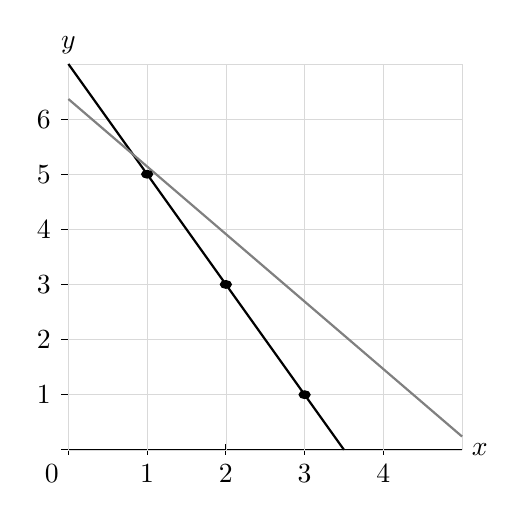
\begin{tikzpicture}[scale=1.0, xscale=1, yscale=0.7]
		\centering
		\draw (0,0) -- (5,0) node[right] {\(x\)};
		\draw (0,0) -- (0,7) node[above] {\(y\)};
		% Add tick marks (optional)

		\foreach \x in {1,2,3,4}
			\draw (\x,0.1) -- (\x,-0.1) node[below] {\x};

		\foreach \y in {1,2,3,4,5,6}
			\draw (0.1,\y) -- (-0.1,\y) node[left] {\y};

		\draw (0,0.1) -- (0, -0.1) node[below left] {0};
		\draw (0.1,0) -- (-0.1, 0) node[below left] {};

		\draw[very thin, gray!30] (0,0) grid (5,7);

		\draw[thick, black, domain=0:3.5] plot (\x, {7 - 2*\x}) node[right] {};
		\draw[thick, gray, domain=0:5.0] plot (\x, {9/sqrt(2) - sqrt(1.5)*\x}) node[right] {};

		\filldraw[black] (3,1) circle (2pt) node[below right] {};
		\filldraw[black] (2,3) circle (2pt) node[above right] {};
		\filldraw[black] (1,5) circle (2pt) node[above left] {};
	\end{tikzpicture}
	\caption{Representación de una capa entera (en negro) junto a un hiperplano afino que no es capa
	entera (en gris). La capa entera tiene como parámetros $\vec{v} = (2, 1)^T$ y $t = 1.4$,
	mientras que los del hiperplano afino son $\vec{v} = (\sqrt{3}, \sqrt{2})^T$ y $t = 1.4$.}
	\label{phase-1:fig:c-layer}
\end{figure}

\begin{lemma}[\cite{herr}]
	Sean $\vec{v}, \vec{x} \in \R^n$ con $\vec{v}$ distinto de cero. Entonces $\vec{x} \in
	H_{\vec{v}, t_{\vec{x}}}$, donde $t_{\vec{x}} \coloneq \frac{\vec{v}^T\vec{x}}{\norm{\vec{v}}^2}$.
\end{lemma}

\begin{theorem}[\cite{herr}]
	\label{phase-1:th:cover}
	Sea $\vec{v} \in \R^n$ un vector esencialmente entero y sea $\vec{w}$ su múltiplo coprimo.
	Entonces la familia de capas enteras $\left\lbrace H_{\vec{w}, k\norm{\vec{w}}^{-2}} \vcentcolon k
			\in \Z \right\rbrace$ cubre a $\Z^n$.
\end{theorem}
\begin{proof}
	% XXX: poner la demostración (?)
\end{proof}

\section{Fase 1: una restricción presupuestaria}

\noindent
Sea $\vec{p} \in \R^n$ un vector esencialmente entero y sea $\vec{q} \in \Z^n$ su múltiplo coprimo.
Consideremos el programa lineal 
\begin{subequations}
	\label{phase-1:formulation}
	\begin{align}
		\max_{\vec{x} \in \Z^n} \quad
			& \vec{p}^T\vec{x}, \label{phase-1:formulation:obj} \\
		\text{s.a.} \quad
			& \vec{p}^T\vec{x} \leq u, \label{phase-1:formulation:c_1} \\
			& \vec{x} \geq \vec{0}. \nonumber
	\end{align}
\end{subequations}

\begin{observation}
	Debido a la restricción presupuestaria (\ref{phase-1:formulation:c_1}), encontramos que el
	politopo está acotado por arriba. Así pues, el problema o bien es infactible, o bien tiene un
	valor óptimo finito.
\end{observation}

Cada escalar $t \in \R$ induce un hiperplano afino $H_{\vec{p}, t}$ donde se cumple que todo punto
$\vec{x} \in H_{\vec{p}, t}$ tiene un mismo nivel de utilidad (\ref{phase-1:formulation:obj}). Como
observamos previamente,
\begin{equation*}
	\left \lbrace H_{\vec{p}, t} \vcentcolon t \in \R \right\rbrace
	=
	\left \lbrace H_{\vec{q}, t} \vcentcolon t \in \R \right\rbrace.
\end{equation*}
A causa del Teorema \ref{phase-1:th:cover}, somos capaces de caracterizar todos los puntos enteros a
partir de $\vec{q}$. Aún más, obtenemos una enumeración de las capas enteras, lo cual nos permite
analizar si la $k$-ésima capa entera contiene puntos factibles para el problema.

Para respetar la restricción presupuestaria (\ref{phase-1:formulation:c_1}), podemos encontrar el
primer\footnote{
	% TODO: explicar a qué me refiero con esto.
} entero $\eta$ que satisfaga $\vec{q}^T\vec{x} \leq u$ para todo $\vec{x} \in H_{\vec{q},
\eta\norm{\vec{q}}^{-2}}$. De esta manera, encontramos que las capas enteras que contienen puntos
enteros que respetan la restricción (\ref{phase-1:formulation:c_1}) son parametrizadas por $k \in
\lbrace \eta, \eta - 1, \ldots \rbrace$.

Ahora bien, para la $k$-ésima capa entera, se cumple que el nivel de utilidad
(\ref{phase-1:formulation:obj}) es $k$. En efecto, si $\vec{x} \in H_{\vec{q},
k\norm{\vec{q}}^{-2}}$, entonces
\begin{equation*}
	\vec{x} = \vec{q}^{\perp} + k\norm{\vec{q}}^{-2}\vec{q},
\end{equation*}
donde $\vec{q}^{\perp}$ es un vector ortogonal a $\vec{q}$. Se cumple inmediatamente que
$\vec{q}^T\vec{x} = k$. De esta manera, deducimos que si la $\eta$-ésima capa entera contiene puntos
no negativos, entonces las soluciones se encuentra en esa capa.

\begin{lemma}
	\label{phase-1:lemma:eta}
	Sea $\vec{p} \in \R^n$ un vector esencialmente entero y sea $\vec{q}$ su múltiplo coprimo, de
	tal manera que $\vec{p} = k\vec{q}$ para algún escalar $k \in \R$. Entonces la primera capa
	entera $H_{\vec{q}, \eta \norm{\vec{q}}^{-2}}$ que satisface la restricción presupuestaria
	(\ref{phase-1:formulation:c_1}) está parametrizada por $\eta \coloneq \lfloor u/k \rfloor$.
\end{lemma}
\begin{proof}
	% TODO: demostrar
\end{proof}

\begin{theorem}
	\label{phase-1:th:feasibility}
	Sea $\vec{p} \in \R^n$ un vector esencialmente entero y sea $\vec{q}$ su múltiplo coprimo.
	Entonces se cumple lo siguiente con respecto al problema (\ref{phase-1:formulation}):
	\begin{enumerate}
		\item El problema es infactible si y solo si $\vec{q} \geq \vec{0}$ y $u < 0$.
		\item Si el problema es factible, su valor óptimo es $\eta$.
	\end{enumerate}
\end{theorem}
\begin{proof}
	% TODO: demostrar
\end{proof}

Supongamos, pues, que el problema (\ref{phase-1:formulation}) tiene solución. Los puntos enteros que
se encuentran en la $\eta$-ésima capa entera satisfacen la ecuación lineal diofantina
\begin{equation}
	\label{phase-1:eq:dioph}
	\vec{q}^T\vec{x} = q_1x_1 + q_2x_2 + \cdots + q_nx_n = \eta.
\end{equation}
En la sección de Teoría de Números mostramos bajo qué condiciones existen soluciones a este tipo de
ecuaciones y también cómo construirlas cuando solamente tenemos dos incógnitas. Por conveniencia
definamos $g_1 \coloneq \gcd{q_1, \ldots, q_n} = 1$ y $\omega_1 \coloneq \eta$. De manera análoga a
una formulación de programación dinámica hacia adelante, podemos definir también
$g_2 \coloneq \gcd{\frac{q_2}{g_1}, \ldots, \frac{q_n}{g_1}}$, con lo que la ecuación anterior es
equivalente a la ecuación
\begin{equation}
	\label{phase-1:eq:forward}
	\frac{q_1}{g_1}x_1 + g_2
		\underbrace{
		\left(\frac{q_2}{g_2 \cdot g_1}x_2 + \cdots + \frac{q_n}{g_2 \cdot g_1}x_n\right)}_{\coloneq
		\omega_2}
	= \omega_1.
\end{equation}
No es difícil observar que $\gcd{\frac{q_1}{g_1}, g_2} = 1$ y por lo tanto existen soluciones
enteras para todo $\omega_1 \in \Z$. Como estos coeficientes son coprimos, encontramos que sus
coeficientes de Bézout asociados (c.f. Definición \ref{prerreq:def:bezout}) $x_1', \omega_2'$ son
soluciones particulares de la ecuación
\begin{equation*}
	\frac{q_1}{g_1}x_1 + g_2\omega_2 = 1,
\end{equation*}
con lo que las soluciones de la ecuación (\ref{phase-1:eq:forward}) están dadas por
\begin{equation*}
	\begin{cases}
		x_1 = \omega_1x_1' + g_2t_1, \\
		\omega_2 = \omega_1\omega_2' - \frac{q_1}{g_1}t_1,
	\end{cases}
\end{equation*}
donde $t_1 \in \Z$. Como la restricción de no negatividad se debe satisfacer ($x_1 \geq 0$),
encontramos que
\begin{equation*}
	t_1 \geq \left\lceil -\frac{\omega_1x_1'}{g_2} \right\rceil.
\end{equation*}
Siguiendo el razonamiento de la formulación dinámica en (\ref{phase-1:eq:forward}), fijamos $t_1$ y
resolvemos la ecuación
\begin{equation*}
	\frac{q_2}{g_2 \cdot g_1}x_2 +
	\frac{q_3}{g_2 \cdot g_1}x_3 +
	\cdots +
	\frac{q_n}{g_2 \cdot g_1}x_n
	= \omega_2.
\end{equation*}
Por construcción, los coeficientes de las incógnitas en el lado izquierdo de la ecuación son
coprimos y por lo tanto existen una infinidad de soluciones para todo $\omega_2 \in \Z$. Por el
mismo razonamiento que el anterior, encontramos que las soluciones son
\begin{equation*}
	\begin{cases}
		x_2 = \omega_2x_2' + g_3t_2, \\
		\omega_3 = \omega_2\omega_3' - \frac{q_2}{g_2 \cdot g_1}t_2,
	\end{cases}
\end{equation*}
donde $t_2 \in \Z$ es un parámetro, $\omega_3$ y $g_3$ están definidos de forma análoga al paso
anterior, y $x_2', \omega_3'$ son los coeficientes de Bézout asociados a $\frac{q_2}{g_2 \cdot g_2}$
y $g_3$, respectivamente. Por la restricción de no negatividad ($x_2 \geq 0$), se debe cumplir
\begin{equation*}
	t_2 \geq \left\lceil -\frac{\omega_2x_2'}{g_3} \right\rceil.
\end{equation*}

De manera general, en el $i$-ésimo paso de la formulación dinámica para $i \in \lbrace 1, \ldots, n
- 2 \rbrace$, encontramos
\begin{equation}
	\label{phase-1:eq:recursive}
	\begin{cases}
		x_i = \omega_ix_i' + g_{i + 1}t_i, \\
		\omega_{i + 1} = \omega_i\omega_{i + 1}' - \frac{q_i}{\prod_{j=1}^{i}g_j}t_i,
	\end{cases}
\end{equation}
donde $t_i \in \Z$ satisface, debido a la restricción de no negatividad,
\begin{equation}
	\label{phase-1:eq:param-bound}
	t_i \geq \left\lceil -\frac{\omega_ix_i'}{g_{i + 1}} \right\rceil.
\end{equation}
Finalmente, en el último paso, obtenemos la ecuación lineal diofantina
\begin{equation}
	\label{phase-1:eq:stopping}
	\frac{q_{n-1}}{\prod_{j=1}^{n-2}g_j}x_{n-1} +
	\frac{q_{n}}{\prod_{j=1}^{n-2}g_j}x_n
	= \omega_{n-1}.
\end{equation}
Nuevamente, los coeficientes de las incógnitas son coprimos. Por lo tanto, las soluciones están
dadas por
\begin{equation}
	\label{phase-1:eq:lastsol}
	\begin{cases}
		x_{n-1} = \omega_{n-1}x_{n-1}' + \frac{q_n}{\prod_{j=1}^{n-2}g_j}t_{n-1}, \\
		x_n = \omega_{n-1}x_n' - \frac{q_{n-1}}{\prod_{j=1}^{n-2}g_j}t_{n-1},
	\end{cases}
\end{equation}
donde ahora $t_{n-1} \in \Z$ debe satisfacer
\begin{equation}
	\label{phase-1:eq:feasible-param}
	\left\lceil -\frac{\omega_{n-1}x_{n-1}'}{q_n} \cdot \prod_{j=1}^{n-2}g_j \right\rceil
	\leq
	t_{n-1}
	\leq
	\left\lfloor \frac{\omega_{n-1}x_n'}{q_{n-1}} \cdot \prod_{j=1}^{n-2}g_j \right\rfloor.
\end{equation}

Como supusimos que el problema es factible (podemos determinar rápidamente si no lo es debido al
Teorema \ref{phase-1:th:feasibility}), existe un vector de parámetros $\vec{t} = (t_1, \ldots,
t_{n-1})$ que satisface las desigualdades (\ref{phase-1:eq:param-bound}) y
(\ref{phase-1:eq:feasible-param}) y por lo tanto que provee una solución al problema
(\ref{phase-1:formulation}). Para encontrar estos parámetros, usamos la técnica de
\textit{backtracking}, en donde hacemos una elección de $t_1, \ldots, t_{n-2} \in \Z$ que satisfaga
(\ref{phase-1:eq:param-bound}) y determinamos si existe $t_n \in \Z$ que satisfaga
(\ref{phase-1:eq:feasible-param}). En caso de que no exista tal parámetro, cambiamos nuestra
elección de $t_1, \ldots, t_{n-2}$. Ciertamente la decisión simple es realizar el cambio $t_{n-2}
\leftarrow t_{n-2} - 1$, aunque también realizar $t_1 \leftarrow t_1 - 1$ puede resultar
beneficioso. Independientemente del caso, eventualmente obtendremos un vector de parámetros $\vec{t}
\in \Z^{n-1}$ que satisfaga las desigualdades necesarias y, por lo tanto, eventualmente obtendremos
un punto entero óptimo.

% TODO: mostrar la comparación con branch and bound.

\section{Fase 2: múltiples restricciones junto con la presupuestaria}
\subsection{Estrategias alternativas para el problema de factibilidad}
\section{Fase 3: múltiples restricciones}
\section{Consideraciones y extensiones del algoritmo}
